\documentclass[../main.tex]{subfiles}
\begin{document}
% \section{Les différentes macros}
\section{命令简介}

% \tkzname{gnuplot} détermine les points nécessaires pour tracer la courbe. Le nombre de points est fixé par l'option \tkzname{samples}; dans les premiers exemples la valeur du nombre de points est celle donnée par défaut. Ensuite  Tikz va utiliser cette table pour tracer la courbe. C'est donc \tkzname{Tikz} qui trace la courbe.
\tkzname{tkz-fct}宏包通过\tkzname{gnuplot}计算函数曲线上的抽样点坐标,
采样点数由\tkzname{samples}选项指定,
在第1个示例中,采样点数取默认值。
得到采样点坐标数据表后,用\TIKZ{}实现绘图。

% \subsection{Tracé d'une fonction avec gnuplot \tkzcname{tkzFct}}
\subsection{\tkzcname{tkzFct}命令:用gnuplot绘制函数曲线}
% Cette première macro est la plus importante car elle permet de tracer la représentation graphique d'une fonction continue .\hypertarget{tfct}{}
该命令是一个重要的命令,用于绘制函数曲线。\hypertarget{tfct}{}

% \begin{NewMacroBox}{tkzFct}{\oarg{local options}\var{gnuplot expression}}
% \emph{La fonction est donnée en utilisant la syntaxe de gnuplot. x est la variable sauf si \tkzname{xstep} est différent de 1, dans ce cas la variable est \tkzcname{x}.}
%
% \medskip
% \begin{tabular}{lll}
% \toprule
%  options             & exemple & explication  \\
% \midrule
% \TAline{gnuplot expression}{x**3}{** représente la puissance $\wedge$}
% \bottomrule
% \end{tabular}
%
% \emph{L'expression est de la forme 2*x+1 ; 3*log(x) ; x*exp(x) ; x*x*x+x*x+x. }
%
% Les options sont celles de \TIKZ.
%
% \begin{tabular}{lll}
% \toprule
% options             & défaut & définition     \\
% \midrule
% \TOline{domain}{xmin:xmax}{domaine de la fonction}
% \TOline{samples}{200}{nombre de points utilisés}
% \TOline{id} {tkzfct}{permet d'identifier les noms des fichiers auxiliaires}
% \TOline{color}{black}{couleur de la ligne}
% \TOline{line width} {1pt}{épaisseur de la ligne}
% \TOline{style} {solid}{style de la ligne}
% \end{tabular}
% \end{NewMacroBox}
\begin{NewMacroBox}{tkzFct}{\oarg{命令选项}\var{gnuplot函数表达式}}
\emph{
函数采用gnuplot语法表示,
其中,x为自变量,如\tkzname{xstep}的值不为1,
则应使用\tkzcname{x}表示自变量。}

\medskip
\begin{tabular}{lll}
\toprule
 参数             & 示例 & 说明  \\
\midrule
\TAline{gnuplot函数表达式}{x**3}{**表示幂运算($\wedge$)}
\bottomrule
\end{tabular}

\emph{类似的函数表达式有:2*x+1、3*log(x)、x*exp(x)、x*x*x+x*x+x等。}

选项可以是所有有效\TIKZ{}选项

\begin{tabular}{lll}
\toprule
选项             & 默认值 & 含义     \\
\midrule
\TOline{domain}{xmin:xmax}{函数定义域}
\TOline{samples}{200}{采样点数}
\TOline{id} {tkzfct}{标识id}
\TOline{color}{black}{颜色}
\TOline{line width} {1pt}{线宽}
\TOline{style} {solid}{线型}
\end{tabular}
\end{NewMacroBox}

% \tkzBomb Lorsque \tkzname{xstep} est différent de $1$, il est nécessaire de remplacer $x$ par |\x|.
\tkzBomb 如果\tkzname{xstep}不为$1$,则自变量$x$需要用|\x|表示。
% \tkzHand Il faut bien évidemment avoir initialisé l'environnement à l'aide  \tkzcname{tkzInit} avant d'appeler \tkzcname{tkzFct}.
\tkzHand 在使用\tkzcname{tkzFct}命令之前,需要用\tkzcname{tkzInit}初始化绘图环境。
% \tkzBomb Attention à ne pas mettre d'espace entre les arguments.
\tkzBomb 参数中不允许留有空白。
%<--------------------------------------------------------------------------->
% \subsection{option : \tkzname{samples}}
\subsection{\tkzname{samples}选项}

如果为线性函数,仅需两个点即可,如
% Il faut remarquer que pour tracer une droite seulement deux points sont nécessaires, ainsi le code~:

\begin{tkzltxexample}[]
\tkzFct[{-(},color=red,samples=2,domain =-1:2]{(8-1.5*\x)/2}
\end{tkzltxexample}


% donne un fichier xxx.table qui contient ~:
生成的\enquote{xxx.table}坐标点数据表的内容为:

\begin{tkzltxexample}[]
# Curve 0 of 1, 2 points
# Curve title: "(8-1.5*x)/2"
# x y type
-1.00000 4.75000  i
2.00000 2.50000  i
\end{tkzltxexample}

% Ce qui est simplement suffisant. Plus simple est dans ce cas, de tracer un segment.
这些数据足够用于绘制简单的线段。

% On demande 400 valeurs pour la table qui va permettre le tracé. Par défaut, la valeur choisie est 200.
以下代码中,为函数曲线设置了400个采样点(\tkzname{samples}选项的默认值是200)。

\medskip
\begin{tkzexample}[latex=7cm]
\begin{tikzpicture}[scale=1]
    \tkzInit[xmax=5,ymax=2]
    \tkzGrid[sub]
    \tkzAxeXY
    \tkzFct[samples=400,domain=.5:5]{1/x}
\end{tikzpicture}
\end{tkzexample}

%<--------------------------------------------------------------------------->
% \subsection{options : \tkzname{xstep, ystep}}
\subsection{\tkzname{xstep, ystep}选项}

\begin{tkzexample}[]
\begin{tikzpicture}
\tkzInit[xmax= 110,xstep=10,
         ymax=6,ystep=1]
\tkzDrawX[label={\textit{年龄}},below= -18pt]
\tkzLabelX
\tkzDrawY[label={\textit{公升s}}]
\tkzFct[domain = 0.1:100 ]{50/\x}
\end{tikzpicture}
\end{tkzexample}


% \subsection{Modification de \tkzname{xstep} et \tkzname{ystep}}
\subsection{改变\tkzname{xstep}和\tkzname{ystep}选项}

% Cette fois le domaine s'étend de 0 à 800, les valeurs prises par la fonction de $0$ à $\numprint{2000}$. \tkzname{xstep=100} donc il faut utiliser |\x| à la place de $x$. Une petite astuce au niveau de gnuplot, 1. et 113. permettent d'obtenir une division dans les décimaux sinon la division se fait dans les entiers.
在此,将函数的定义域设置为$0$到$\numprint{700}$,并取\tkzname{xstep=100},
值域设置为$0$到$\numprint{2000}$。
因此,在函数表达式中应该用|\x|代替$x$。
注意,在gnuplot中,需要使用类似\enquote{\tkzname{1.}}和\enquote{\tkzname{113.}}
带\tkzimp{小数点}的数字进行浮点数除法运算,
否则,则会使用整数除法运算(例如1/3的结果为0)。

% Ensuite, j'utilise les macros pour placer des points
然后,用该命令绘制函数曲线。
%<--------------------------------------------------------------------------->
\begin{tkzexample}[vbox]
\begin{tikzpicture}[scale=1.5]
 \tkzInit[xmax=700,xstep=100,ymax=1200,ystep=400]
 \tkzGrid(0,0)(700,1200)  \tkzAxeXY
 \tkzFct[color=red,samples=100,line width=0.8pt,domain =0:700]%
        {(1./90000)*\x*\x*\x-(1./100)*\x*\x+(113./36)*\x}
\end{tikzpicture}
\end{tkzexample}

% \subsection{\tkzname{ystep} et les fonctions constantes}
\subsection{\tkzname{ystep}选项和常函数}

% Attention, ici  \tkzname{ystep=6} or \tkzname{gnuplot} donne $80\div 6=13$. il faut donc écrire $80.$
在此\tkzname{ystep=6},由于\tkzname{gnuplot}执行$80\div 6$运算的结果是$13$。
因此,应该使用\enquote{$80.0$}表示常函数。



\begin{tkzexample}[vbox]
 \begin{tikzpicture}[scale=0.4]
 \tkzInit[xmax=30,ymax=90,ystep=6]
 \tkzDrawX[right,label=$t$]
 \tkzDrawY[above,label=$P$]
 \tkzFct[line width=1pt,color=red,dashed,domain=0:30]{80.0}
 \tkzFct[line width=1pt,color=blue,domain=0:30]{80/(1.0+4.0*exp(-0.21*x))}
 \tkzText[above,color=red](20,80){$P=80$}
\end{tikzpicture}
\end{tkzexample}

% \subsection{Les fonctions affines ou linéaires}
\subsection{仿射函数或线性函数}
% Pour obtenir des droites, on peut utiliser \tkzname{gnuplot} même si l'outil est un peu lourd dans ce cas. Pour alléger les calculs, il est possible de ne demander que deux points !
可以使用\tkzname{gnuplot}绘制直线,虽然这样会增加绘图负担,为简化计算,可只使用2个采样点。

\begin{tkzexample}[vbox]
 \begin{tikzpicture}[]
 \tkzInit[ymax=20,ystep=5]
 \tkzAxeXY
 \tkzFct[color=red,domain=0:10,samples=2]{2*x+5}
 \tkzFct[color=blue,domain=0:10,samples=2]{-x+15}
 \tkzFct[color=green,domain=0:10,samples=2]{7} % 7/5=1(整数)
 \tkzFct[color=purple,domain=0:10,samples=2]{7.}%7.0/5 =1.2(浮点数)
\end{tikzpicture}
\end{tkzexample}
   %<--------------------------------------------------------------------------->
\subsection{子网格}

   $y=(x-4)\text{e}^{-0.25x+5}$

% Il est possible de dessiner une autre grille.
可以采用子网格突出表示函数曲线局部。

\begin{tkzexample}[latex=8cm]
\begin{tikzpicture}
 \tkzInit[xmin=4,xmax=18,xstep=2,
          ymin=20,ymax=90,ystep=10]
 \tkzFct[domain = 5:18]%
        {(\x-4)*exp(-0.25*\x+5)}
 \tkzGrid(4,20)(18,90)
 \tkzAxeXY
 \tkzGrid[sub,
          subxstep=0.5,
          subystep=2,
          color=brown](6,60)(12,90)
\end{tikzpicture}
\end{tkzexample}
%<--------------------------------------------------------------------------->
\subsection{使用\tkzname{tkz-base}宏包的命令}
% Toutes les macros de  \tkzname{tkz-base} sont bien sûr utilisables, en voici quelques exemples.
在绘图中,也可以直接使用\tkzname{tkz-base}宏包的命令。

\begin{center}
	\begin{tkzexample}[vbox]
	\begin{tikzpicture}[scale=2]
	 \tkzInit[xmin=-3,xmax=3, ymin=-1,ymax=4]
	 \tkzGrid[sub,subxstep=.5,subystep=.5]
	 \tkzAxeXY
	 \tkzFct[domain = -3:2]{(2-x)*exp(x)}
	 \tkzText(-2,1.25){$\mathcal{C}_{f}$}
	 \tkzDefPoint(2,0){A} \tkzDrawPoint(A)  \tkzLabelPoints(A)
	 \end{tikzpicture}
	\end{tkzexample}
\end{center}


%<--------------------------------------------------------------------------->
\end{document}
\endinput
